%\documentclass[a4paper,11pt,leqno,notitlepage,onecolumn]{article}
\documentclass[a4paper,11pt,leqno,notitlepage,twocolumn]{article}

\usepackage[latin1]{inputenc}
\usepackage{fontenc}
\usepackage{graphicx}
\usepackage[dvips]{hyperref}

\usepackage{setspace}
%\doublespacing

\begin{document}
\title{Efficient Static Binary Instrumentation in the Presence of Variable-Length Instructions}
\author{Michael Laurenzano, Mustafa Tikir, Laura Carrington, Allan Snavely\\
San Diego Supercomputer Center\\
\it{\{michaell, mtikir, laurac, allans\}@sdsc.edu}}
\date{}
\maketitle

\begin{abstract}
\begin{it}

Binary instrumentation facilitates the insertion of additional code into an
executable in order to observe or modify the behavior of application runs. 
There are two main approaches to binary instrumentation: static and dynamic
binary instrumentation. In this paper we present PMaC's instrumentation toolkit, PIX, 
an efficient static instrumentation toolkit for Linux on x86/x86\_64 platforms. PIX
is similar to  other toolkits in terms of how additional code is inserted. However, it uses function-level
code relocation in order to remedy the difficulty created by the underyling variable-length instruction set. 
Code relocation of this kind allows the reorganization of the application code in such a way that it
can use fast far-reaching constructs to transfer control
from the application to the instrumentation code rather than relying on multiple
jumps or interrupts. Furthermore, the PIX API provides 
tool developers means to insert lightweight hand-coded assembly
rather than relying solely on the insertion of entire instrumentation functions.
Because of these features PIX enables implementation of efficient instrumentation tools. 
The overhead imposed by a simple basic block counting tool created using PIX is an
average of 1.6x less than the overhead imposed by Pin, 4.7x less than the overhead imposed by
DynamoRIO, 7.8x less than the overhead imposed by Valgrind, and 10x less than the overhead imposed by Dyninst.

\end{it}

\end{abstract}

\label{Section:Introduction}
\section{Introduction}
\section{Introduction}
\label{sec:Introduction}

Binary instrumentation toolkits can be used to insert additional code into an
executable in order to observe or modify the behavior of application runs.
Instrumentation toolkits such as Pin\cite{luk2005pin},
Dyninst\cite{buck2000api}, Valgrind\cite{nethercote2007valgrind} and
DynamoRIO\cite{bruening2004efficient} have been widely used to gather
information about application runs. It has been shown that data gathered from
instrumentation tools can be effectively used in guiding hardware and system
design\cite{uhlig1997trace}, program debugging and
correctness\cite{nethercote2007shadow}, program
optimization\cite{romer1997instrumentation}, security
verification\cite{miller-playing}, and performance
modeling/prediction\cite{snavely2001modeling}.

There are two main approaches to binary instrumentation: \textit{static} and
\textit{dynamic} binary instrumentation. Static binary instrumentation inserts
additional information into an executable and generates a persistent modified
executable whereas the dynamic instrumentation inserts additional information
during execution without making any permanent modifications to the executable.
The static instrumentation approach can be advantageous because it usually
results in more efficient executables when compared to the dynamic approach.
This is a result of the fact that static instrumentation introduces only the
instrumentation code itself, which is also included in the text section of the
executable. In dynamic binary instrumentation, additional overhead is introduced
because the instrumentation tool must perform additional tasks such as parsing,
disassembly, code generation, and making other decisions at runtime.

This is simply not an issue with static binary instrumentation tools because all
decisions and actions are taken prior to runtime. The only cost born at runtime
is the direct cost of performing additional instrumentation. Unlike static
instrumentation, dynamic instrumentation uses the program heap for the
instrumentation code and hence, use the data section as text space. However,
static binary instrumentation has disadvantages. It is not possible to
instrument shared libraries unless the shared libraries are instrumented
separately and the executable is modified to use those instrumented libraries.
Static instrumentation also provides less flexibility to tool developers since
any instrumentation code that is inserted persists throughout the application
run while dynamic instrumentation provides the means to delete instrumentation
code when it is not needed \cite{tikir2002efficient}. However, there are cases
where the importance of efficiency is enough to outweigh other shortcomings
\cite{carrington2006performance} so that static binary instrumentation is the
desirable paradigm.   

In this paper we introduce \textbf{P}MaC's \textbf{E}fficient static
\textbf{B}inary \textbf{I}nstrumentation toolkit for \textbf{L}inux on
x86/x86\_64, \textit{PEBIL}. The goal of PEBIL is to provide a toolkit that
enables the construction of instrumentation tools that produce an efficient
instrumented executable. More specifically, PEBIL is designed to generate
efficient instrumented executables for instrumentation tools that require a
large number of instrumentation points because these are the situations where
efficiency is expected to be most impacted. Similar to previous instrumentation
toolkits \cite{buck2000api}, PEBIL instruments the executable by placing a jump
instruction at each instrumentation point in the application which transfers
control to the instrumentation code. This instrumentation code saves program
state, performs tasks requested by the instrumentation tool, restores program
state, and then returns control to the application. A typical binary
instrumentation tool on a platform with fixed-length instructions
\cite{tikir2006pmac} accomplishes initial control transfer by replacing a single
instruction at the instrumentation point with a jump that transfers control to
the instrumentation code. 

When instructions are variable-length, however, this strategy is not always
possible since there may not be enough space to correctly insert such a jump
instruction. To address this, PEBIL relocates and tranforms the code for each
function to ensure that enough space (in the form of \begin{it}nops\end{it}) is
available to hold a full-length branch instruction at each instrumentation
point. This method of function relocation enables transformation of the code so
that it can use longer-range yet efficient jump instructions to transfer control
from the application to the instrumentation code. Similar to Dyninst
\cite{buck2000api}, PEBIL uses the concept of an instrumentation
\textit{snippet}, which is a lightweight hand-written body of assembly code that
can be used to perform instrumentation tasks, rather than relying only on
heavyweight instrumentation functions.

The PEBIL toolkit, along with other accompanying tools and documentation, is
open source and available to the public for download at
\url{http://blind-review-forbids-real-urls.com/}. The distribution includes
several instrumentation tools including a function execution counter, a basic
block execution counter, and a memory address stream collection tool. Each of
these tools is built on top of an API that provides both enough low-level detail
to allow the tool developer to get involved in the details of the
instrumentation and enough high-level capability to allow the tool builder to
ignore these details if he wishes. The three instrumentation tools provided with
the distribution are implemented in less than 600 lines of C++ code. The
remainder of the paper is organized as follows. Section \ref{sec:Overview}
describes the design and implementation of PEBIL. Section \ref{sec:Efficiency}
discusses several aspects of the toolkit that are related to efficiency,
including the function relocation mechanism and the instrumentation snippet.
Section \ref{sec:Results} presents some experiments that expose the performance
penalties imposed by instrumenting applications with PEBIL, as well as a
comparison of PEBIL to other state of the art binary instrumentation toolkits
for x86 including Dyninst, Pin, Valgrind and DynamoRIO. Section \ref{sec:Future}
discusses the future of PEBIL, Section \ref{sec:Related} discusses other popular
instrumentation tools related to PEBIL and Section \ref{sec:Conclusions}
concludes.


\label{Section:Implementation}
\section{Implementation}
%\input{implementation}

\label{Section:Relocation}
\section{Relocation}
The novel use of relocation in our instrumentation strategy stems from the fact that we are performing
the instrumentation statically on a platform that uses a variable-length instruction
set. A typical strategy used by static instrumentation tools on platforms with 
fixed-length instruction sets is to replace a single fixed-length instruction at 
the instrumentation point with a branch instruction that will transfer control to 
the code produced by the instrumentation tool. This is fairly straightforward to
do because by the definition of a fixed-length instruction set,
the instruction being replaced and the replacement branch have the same length. Performing
static instrumentation in a variable-length instruction set does not afford us this luxury.
In X86, an unconditional branch that uses a 32-bit offset requires 5 bytes, whereas some
of the instrumentation points that interest us may use only a single byte.

This leaves two options for how to transfer control to the instrumentation code. We must either use 
a technique entirely distinct from the idea of using a single unconditional branch to execute the control
transfer such as multiple shorter jumps or software interrupts, or we must somehow alter the
application code so that it can accomodate a single large control instruction that is larger than the original
amount of space available at the instrumentation point. A seperate technique for transferring control flow
could be to use a series of branches, where the instruction in the instrumentation point is a small branch that
transfers control to a larger intermediate branch. We do not consider this method any further because the smallest
unconditional branch instruction is 2 bytes in length, making it ultimately a half measure since there are instrumentation
points with only a single byte available to them. Another option to consider is the method proposed by the BIRD project 
\ref{nanda2006bird}. They propose using the single-byte \begin{it}INT 3\end{it}
instruction, a single-byte interrupt intended to be used by debuggers to set breakpoints, when a larger branch won't fit within 
the specified area. This instructions is functionally perfect for static instrumentation because it consumes only a single
byte and allows us to transfer control to an arbitrary location by registering an exception handler
with the system. We performed a cursory study on this scheme from an efficiency standpoint to determine whether it was worth
further investigation. On a small benchmark set, our
implementation of using \begin{it}INT 3\end{it} only when 5-byte unconditional branches do
not fit at the instrumentation point introduces slowdowns of no less than 100-fold for counting the
number of executions of each basic block in the code. As one might expect, this mechanism is unsuitable
for efficient instrumentation because the very heavyweight system call conventions are being invoked
fairly often.

We use the latter option, reorganizing the code at the function level so that there is enough space at every instrumentation
point to accomodate a 5-byte branch. Specifically, the steps we use are as follows:
\begin{enumerate}
\item 
1. Function Displacement
\item
2. Link Function Entries 
\item
3. Branch Conversion
\item
4. Instruction Padding
\end{enumerate}


Figure \ref{Figure:Relocation} gives a visual version of this process.

1. Function Displacement: Relocate the contents of the entire function to an area of the text section allocated
to the instrumentation tool. Since functions are often packed tightly together, it is generally not possible to
expand the size of a function without disturbing the entry points of another function.

2. Link Function Entries: Place an unconditional branch at the former function entry point that transfers control
to the new function entry point. Most references to the entry point of a function are in the form of function calls, which
routinely are indirect references (ie their value is computed or looked up at runtime) and are difficult to resolve
prior to runtime.

3. Branch Conversion: Convert each short conditional branch in the relocated function to the equivalent
5-byte branch instruction. Since the code is being reorganized in the next step which may strain the limits of
smaller 8-bit or 16-bit offsets, we convert all branches to use 32-bit offsets so that the targets of each branch
will still be reachable without having the need to further reorganize the code. Note that there is some opportunity
here to reduce space by using the smallest branch offset size that accomodates the branch, but this is an issue
for future work.

4. Instruction Padding: According to the needs of the instrumentation tool, pad the instruction at each instrumentation
point with \begin{it}nop\end{it} instructions so that a 5-byte branch can fit.

There are several ways that this process can adversely affect the performance of the application independant of the overhead
that will be imposed by inserting any extra instrumentation code. Each function call
now has an extra control interruption associated with it since control must be passed first to the original function entry
point and then to the relocated function entry point. It is possible that using 32-bit offsets for every branch rather than
some smaller number of bits has an overhead associated with it. And since the code is being reorganized and expanded, 
we might destroy some positive alignment and size optimizations that the compiler might have made on the instructions in the
function. We examine the practical overhead seen by these techniques by taking these steps without instrumenting the code
for a series of benchmarks. The slowdown is XXXX...


\label{Section:Coverage}
\section{Coverage}
\subsection{Code Coverage}
Code and data can reside together in the text section of a program binary. This is done for a variety of reasons, including
the storage of branch target locations (eg for a jump table) or small data structures that provide convenient lookup
of certain data such as identifiers, descriptors, or other values.

Correctly determining
what parts of the text sections are code and what are data is important. Consider what can happen
if we mistakenly treat some data as code. We might choose to modify or relocate the apparent code
to serve our instrumentation purposes. Then when the data at this location is referenced, the
original program behavior may not be preserved: if we are lucky this will cause application failure
due to some unexpected change in control flow or some state condition that is checked by the program.
If we are unlucky the corruption might silently manifest itsself by modifying the output of the
program. Alternatively consider what can happen if we mistakenly treat some code as data. We then will
not try to insert code into this area or we might perform some other type of analysis that should be reserved for
data alone. While this is almost certainly preferrable to the situation where we treat data as code, it
is ideal to avoid both situations.

To this end, we use the program's symbol table to help us determine which parts of the text sections
are functions that are eligible to be subject for our code discovery algorithm. Our code discovery algorithm
consists of two phases; control-driven disassembly backed up by linear disassembly. In more detail, the algorithm
works as follows:

\begin{enumerate}
\item 
1. Control-driven disassembly: from a function's entry point, follow all understandable control paths. If a problem is encountered, fall back to
naive disassembly.

2. Naive disassembly: from a function's entry point, disassemble each instruction in the order it appears in the
function. If a problem is encountered, give up.
\end{enumerate}


Problems that can be encountered are situations where an unknown opcode is encountered, where control jumps to the
middle of an instruction we've already disassembled, or if control leaves the boundaries of the function. In most
cases control-driven disassembly is sufficient to disassemble the entirety of a function, and in most cases control-driven
disassembly is a straightforward process because control either falls through to the following instruction 
or the location of a branch target is embedded entirely within the instruction itsself. But there are also cases
where the an indirect branch is used, where the target resides either at a fixed address (possibly with some offset), the address that resides in a register,
or the address that is at a location given by a register. The latter two cases are very difficult to resolve
without runtime information because the computation of the target address can be arbitrarily complex and can span function
boundaries. Nevertheless, we perform a poophole examination of the previous instructions to the and can determine 
the address in simple cases.

Fortunately simple calculations are all that most compilers use to determine targets for jump tables, one of the more common
uses of an indirect branch. Often an offset is added to a fixed location to determine where the data comprising the branch target
resides. Therefore we treat such a fixed address as the first entry in a table whose entries are treated either as addresses or as offsets.
We then make an iterative pass over this table to determine the target for each arm of the jump table, stopping when we find a value in the
table that yeilds an address that is outside the scope of the function.

 PUT EXAMPLE OF GNU COMPILER JUMP TABLE HERE



\label{Section:Snippets}
\section{Snippets}
%\input{snippets}

\label{Section:Results}
\section{Results}
%\section{Results}
\label{sec:Results}

The main design goal of PEBIL is to generate efficient instrumented code. 
To investigate the efficiency of instrumented executables created by PEBIL, we ran several experiments 
on a selection of benchmarks from the the SPEC CPU2000 Integer benchmark suite comprised of
bzip2, crafty, gap, gzip, mcf, parser, perlmbk, twolf, vortex and vpr. All of the experiments are run on a
single core of a quad-core 2.4GHz IA32 Intel Xeon running Red Hat Linux Enterprise 4.1.2 (Linux kernel 2.6.18). 

The first set of experiments quantifies the overhead of the program relocation and 
transformation techniques used by PEBIL and
described in Section \ref{Subsection:Relocation}. 
Recall that this technique adds an additional unconditional
branch execution to each function call in order to relocate the function, extends all of the branches in the code
to use 32-bit offsets, and pads each basic block whose size is fewer than 5 bytes with nops so that a
5 byte jump to the instrumentation code can be inserted. These transformations are performed on our benchmark set 
so that the code is ready for the insertion of instrumentation code but is not actually instrumented. 

Figure \ref{fig:RelocOverhead} presents
the runtime overhead seen in the instrumentation-ready executables as a percentage of the original application runtime.
The figure shows that the maximum overhead due to these modifications is 6.5\%, with an
average overhead of just 1.6\%. Among a set of popular dynamic instrumentation toolkits,
Pin, DynamoRIO and Valgrind, the lowest overhead for running the application within the instrumentation
tool but performing no instrumentation
on the IA32 platform is obtained by using DynamoRIO. DynamoRIO has an average of 38\% overhead and a maximum overhead of 113\% on
our SPEC CPU2000 Integer benchmark set \cite{luk2005pin}. This shows that the 
relocation and transformation method used by PEBIL has a minimal
performance impact on the performance of these benchmarks and thus is a suitable approach as a basis for
producing efficient instrumented code.

\begin{figure}[ht]
\centering
\label{fig:RelocOverhead}
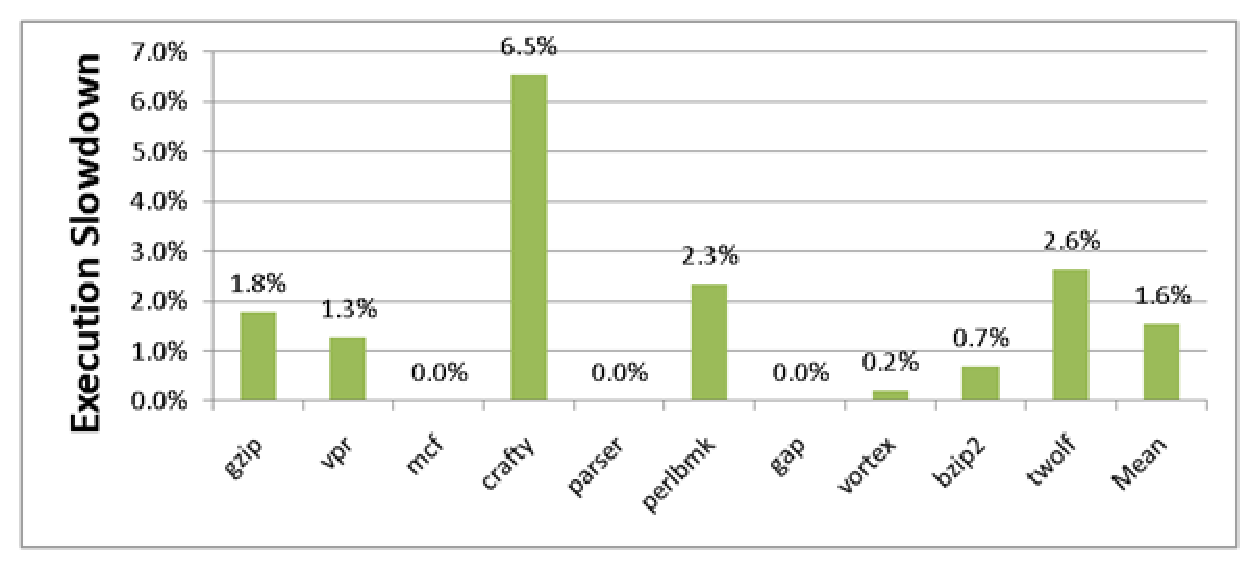
\includegraphics[scale=0.6]{relocperf.eps}
\caption{Application overhead caused by preparing the code for instrumentation but without
any instrumentation inserted.}
\end{figure}

The next set of experiments shows how much overhead is introduced due to counting the
basic block executions in the application. We use this particular instrumentation tool because basic block counting
is an example of an instrumentation tool where we would expect PEBIL to generate efficient instrumented executables
as the number of instrumentation points required is high. Much of the work performed in basic block counting, namely updating a single
counter every time a basic block is encountered, can be done easily using a fast instrumentation snippet rather than
by a full instrumentation function. The counters embodied in the instrumentation snippets must also be
persistent throughout the entire run of the application, which is more suited to a static instrumentation approach
because the static instrumentation does not utilize any resources to determine whether instrumentation can be removed.
The basic block counting instrumentation tool is used to produce an instrumented
executable for each program in our benchmark suite, whose runtime is compared to the runtime of the 
unmodified original executable. The results of these experiments are shown in Figure \ref{fig:ToolOverheads}. 

\begin{figure}[ht]
\centering
\label{fig:ToolOverheads}
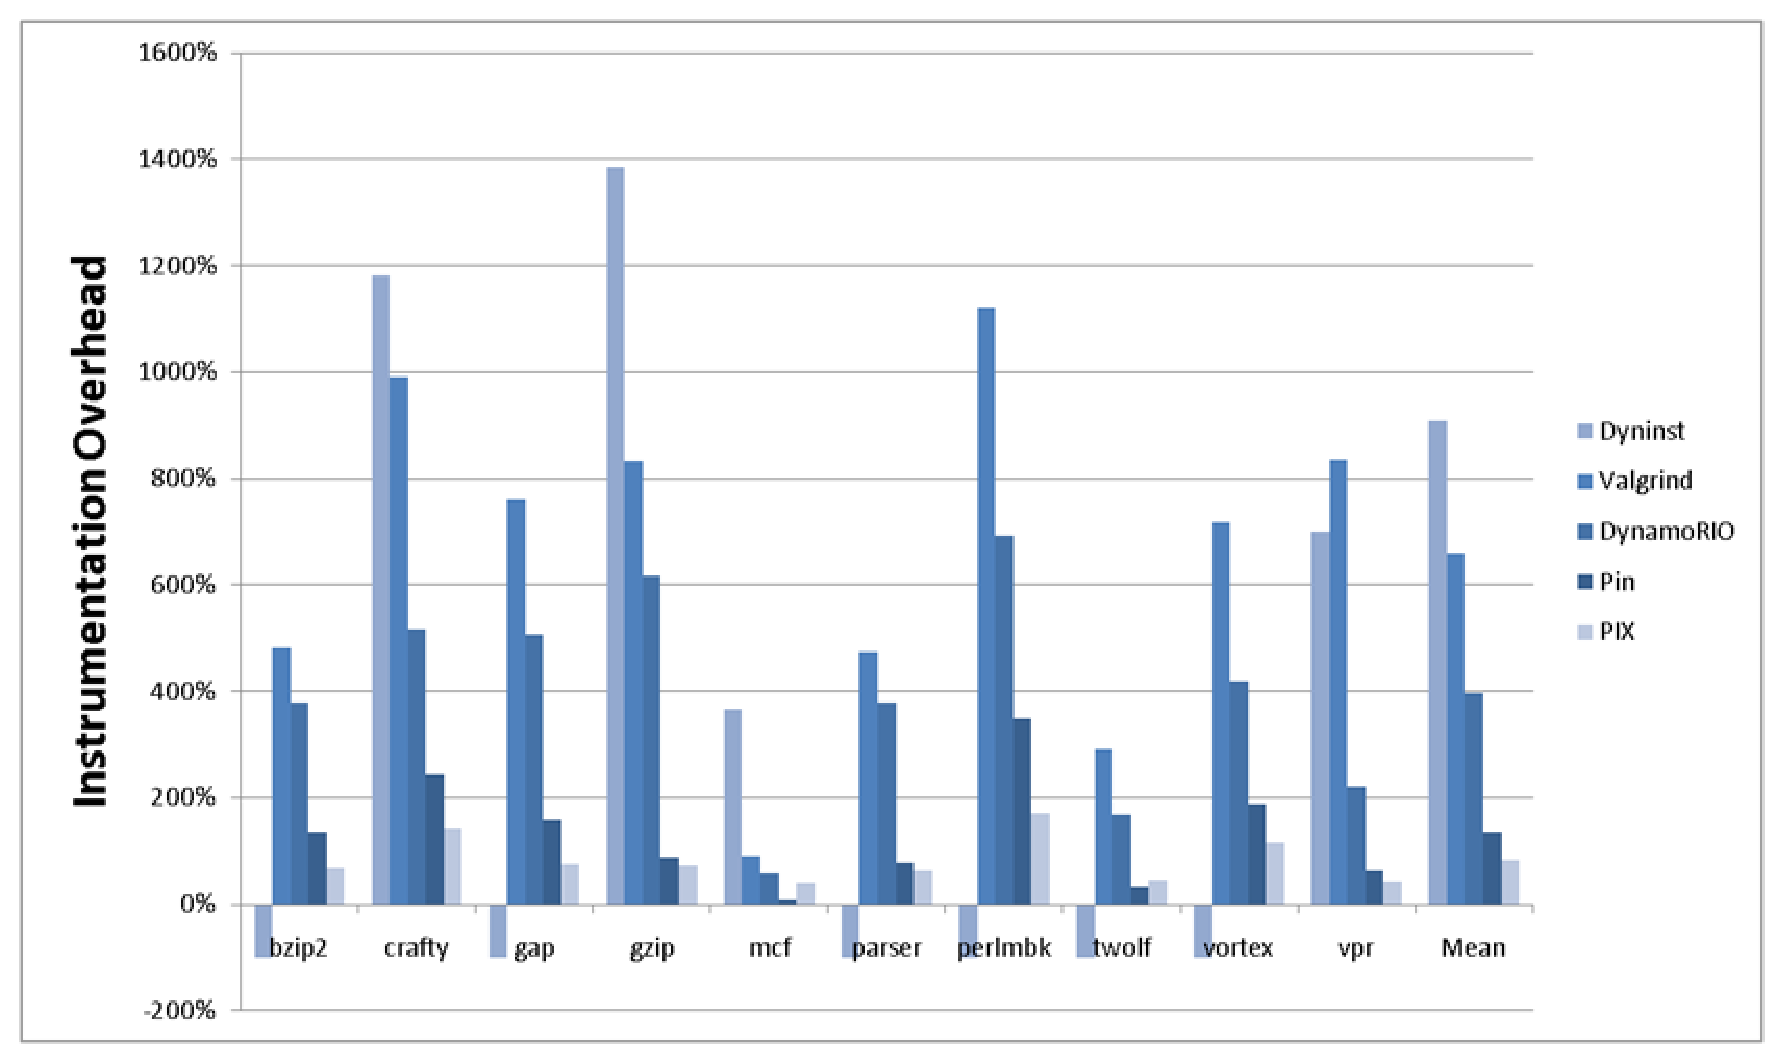
\includegraphics[scale=0.32]{bbcount.eps}
\caption{Performance of several x86 instrumentation tools with basic block counting instrumentation.}
\end{figure}

Figure \ref{fig:ToolOverheads} presents the overhead introduced as a percentage of the original application runtime. The
overhead of PEBIL's basic block counter ranges from 41\%-170\% for the benchmarks tested with an average overhead of 
84\%. More importantly, the figure shows that the overhead introduced by PEBIL instrumentation is significantly 
lower than those introduced by the other instrumentation toolkits available for the x86 platform. 
The average overhead is 135\% for Pin (ranging from 8\%-350\%), 
396\% for DynamoRIO (ranging from 58\%-693\%), 660\% for Valgrind (ranging from 91\%-1120\%), 
and 1936\% for Dyninst (ranging from 367\%-7859\%). Note also that, like PEBIL, the Dyninst
implementation of a basic block counter uses snippet-based instrumentation whenever possible yet
it results in significantly higher overheads than PEBIL.
Our experiments demonstrate that executables instrumented by PEBIL run an average of
51\% faster than the next most efficient instrumentation toolkit for basic block counting, Pin. Furthermore,
Pin uses a variety of optimizations such as tracking eflags bit liveness \cite{luk2005pin} that are currently
unincorporated into PEBIL. We plan to incorporate more optimizations to PEBIL in the future (see Section \ref{sec:Future}) including
several optimizations already in use by Pin, which should further improve the efficiency of the instrumented
executables generated by PEBIL.



\label{Section:Future}
\section{Future}
\section{Future Work}
\label{sec:Future}

Despite the success in terms of efficiency, there are several additional techniques
that might make the instrumented code even more efficient in PIX. Because PIX relocates
the text to yeild extra space for the manipulation of the application functions, 
rather than inserting just a branch
that transfers control to the instrumentation code we have the opportunity to inline
the instrumentation code itsself
in order to reduce or eliminate the control interruptions  that otherwise must be taken 
when inserting the instrumentation code.

Currently PIX saves all general purpose registers around each function call and allows the
tool developer to state which registers are saved around instrumentation snippets. For even more efficient instrumentation
snippets, we could automatically detect which registers are killed by the instrumentation code and which are live at the entry point
of the instrumentation code, and automatically save only the ones that are alive. Similarly, we could perform register 
analysis in order to identify the instrumentation points where the machine state doesn't need to be saved around instrumentation functions. 

Finally, similar to Pin, we could perform liveness on the bits of the eflags/rflags register to determine whether the flag registers need to be saved and
restored at each instrumentation point. Optimizations that help PIX avoid saving and restoring state at each instrumentation point 
have the potential to further the overhead associated with instrumentation and we beleive 
that they will further the goal of generating efficient instrumented code with PIX.




\label{Section:Conclusions}
\section{Conclusions}
%\section{Conclusions}



\bibliography{paperbib}
\bibliographystyle{unsrt}

\end{document}

